\documentclass{article}

% Language setting
% Replace `english' with e.g. `spanish' to change the document language
\usepackage[english]{babel}

% Set page size and margins
% Replace `letterpaper' with `a4paper' for UK/EU standard size
\usepackage[letterpaper,top=2cm,bottom=2cm,left=3cm,right=3cm,marginparwidth=1.75cm]{geometry}

% Useful packages
\usepackage{amsmath}
\usepackage{graphicx}
\usepackage[colorlinks=true, allcolors=blue]{hyperref}
\usepackage{xcolor}
\usepackage{datetime}
\usepackage[section]{placeins} 
\usepackage{pdfpages}
\usepackage{float}

\title{ME136 Lab 4}
\author{Nathan Yacovetta, Aarchan Saxena, Jobanpreet Mutti, Radhika Marolia}
\date{November 2, 2023}

\begin{document}
\maketitle

\section{Contributions}

\begin{itemize}
\item Nathan Yacovetta: Analyzed data and worked on the deliverables including all the Matlab code to make the plots.
\item Aarchan Saxena: Performed the lab tasks and virtual machine code, and worked on deliverables. 
\item Jobanpreet Mutti: Worked on the deliverables and report write up.
\item Radhika Marolia: Worked on the deliverables and report write up.
\end{itemize}

\section{Experimental Set-up:}
\subsection{Description}
We mount the vehicle on the rotational rig shown in the table below. This rotational rig connects the drone on one horizontal axis so that it is only able to rotate in the pitch direction. This allows us to test different pitch angles without damaging the vehicle. 


\subsection{Screenshots}
\begin{table}[ht] 
\centering 
\begin{tabular}{|c|c|} 
\hline 
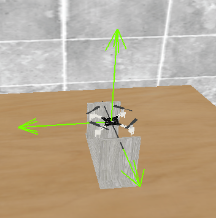
\includegraphics[width=0.4\textwidth]{Screenshot 2023-11-01 201709.png} & 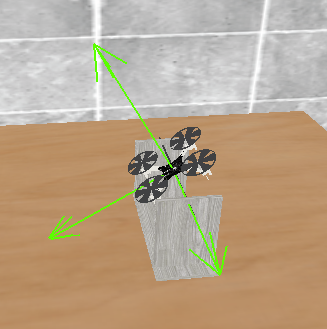
\includegraphics[width=0.4\textwidth]{Screenshot 2023-11-01 201609.png} \\ 
\hline 
\end{tabular} 
\caption{Experimental Set-Up} 
\label{tab:images} 
\end{table} 

\section{Mixer Equations and Code}

\begin{align}
\begin{bmatrix}
c_{P1}\\[1ex]
c_{P2}\\[1ex]
c_{P3}\\[1ex]
c_{P4}
\end{bmatrix} = .25
\begin{bmatrix}
1 & \frac{1}{L} & -\frac{1}{L} & \frac{1}{k}\\[1ex] 
1 & -\frac{1}{L} & -\frac{1}{L} & \frac{1}{k}\\[1ex] 
1 & -\frac{1}{L} & \frac{1}{L} & \frac{1}{k}\\[1ex] 
1 & \frac{1}{L} & \frac{1}{L} & -\frac{1}{k}
\end{bmatrix}
\times 
\begin{bmatrix}
c_{\sum}\\
n_1\\
n_2\\
n_3
\end{bmatrix}
\end{align}

Here $c_{pi}$ represents the thrust of each individual propeller in Newtons. L is the perpendicular distance of the propellers in meters to the axes spanning the body fixed transverse plane. k is the coupling coefficient in meters. $n_i$ is the moment (N*m) around the i body fixed axis. The implementation can be seen below. 

\begin{figure} [H]
\centering
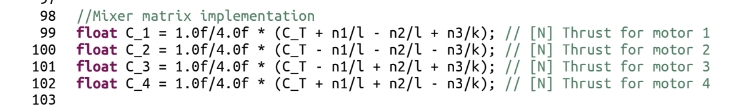
\includegraphics[scale=.8]{MMI.png}
\caption{Implementatoin of Mixer Matrix }
\end{figure}
\FloatBarrier
\vspace{24pt}

\section{Step Input Response}
\subsection{Part A}
\begin{figure} [H]
\centering
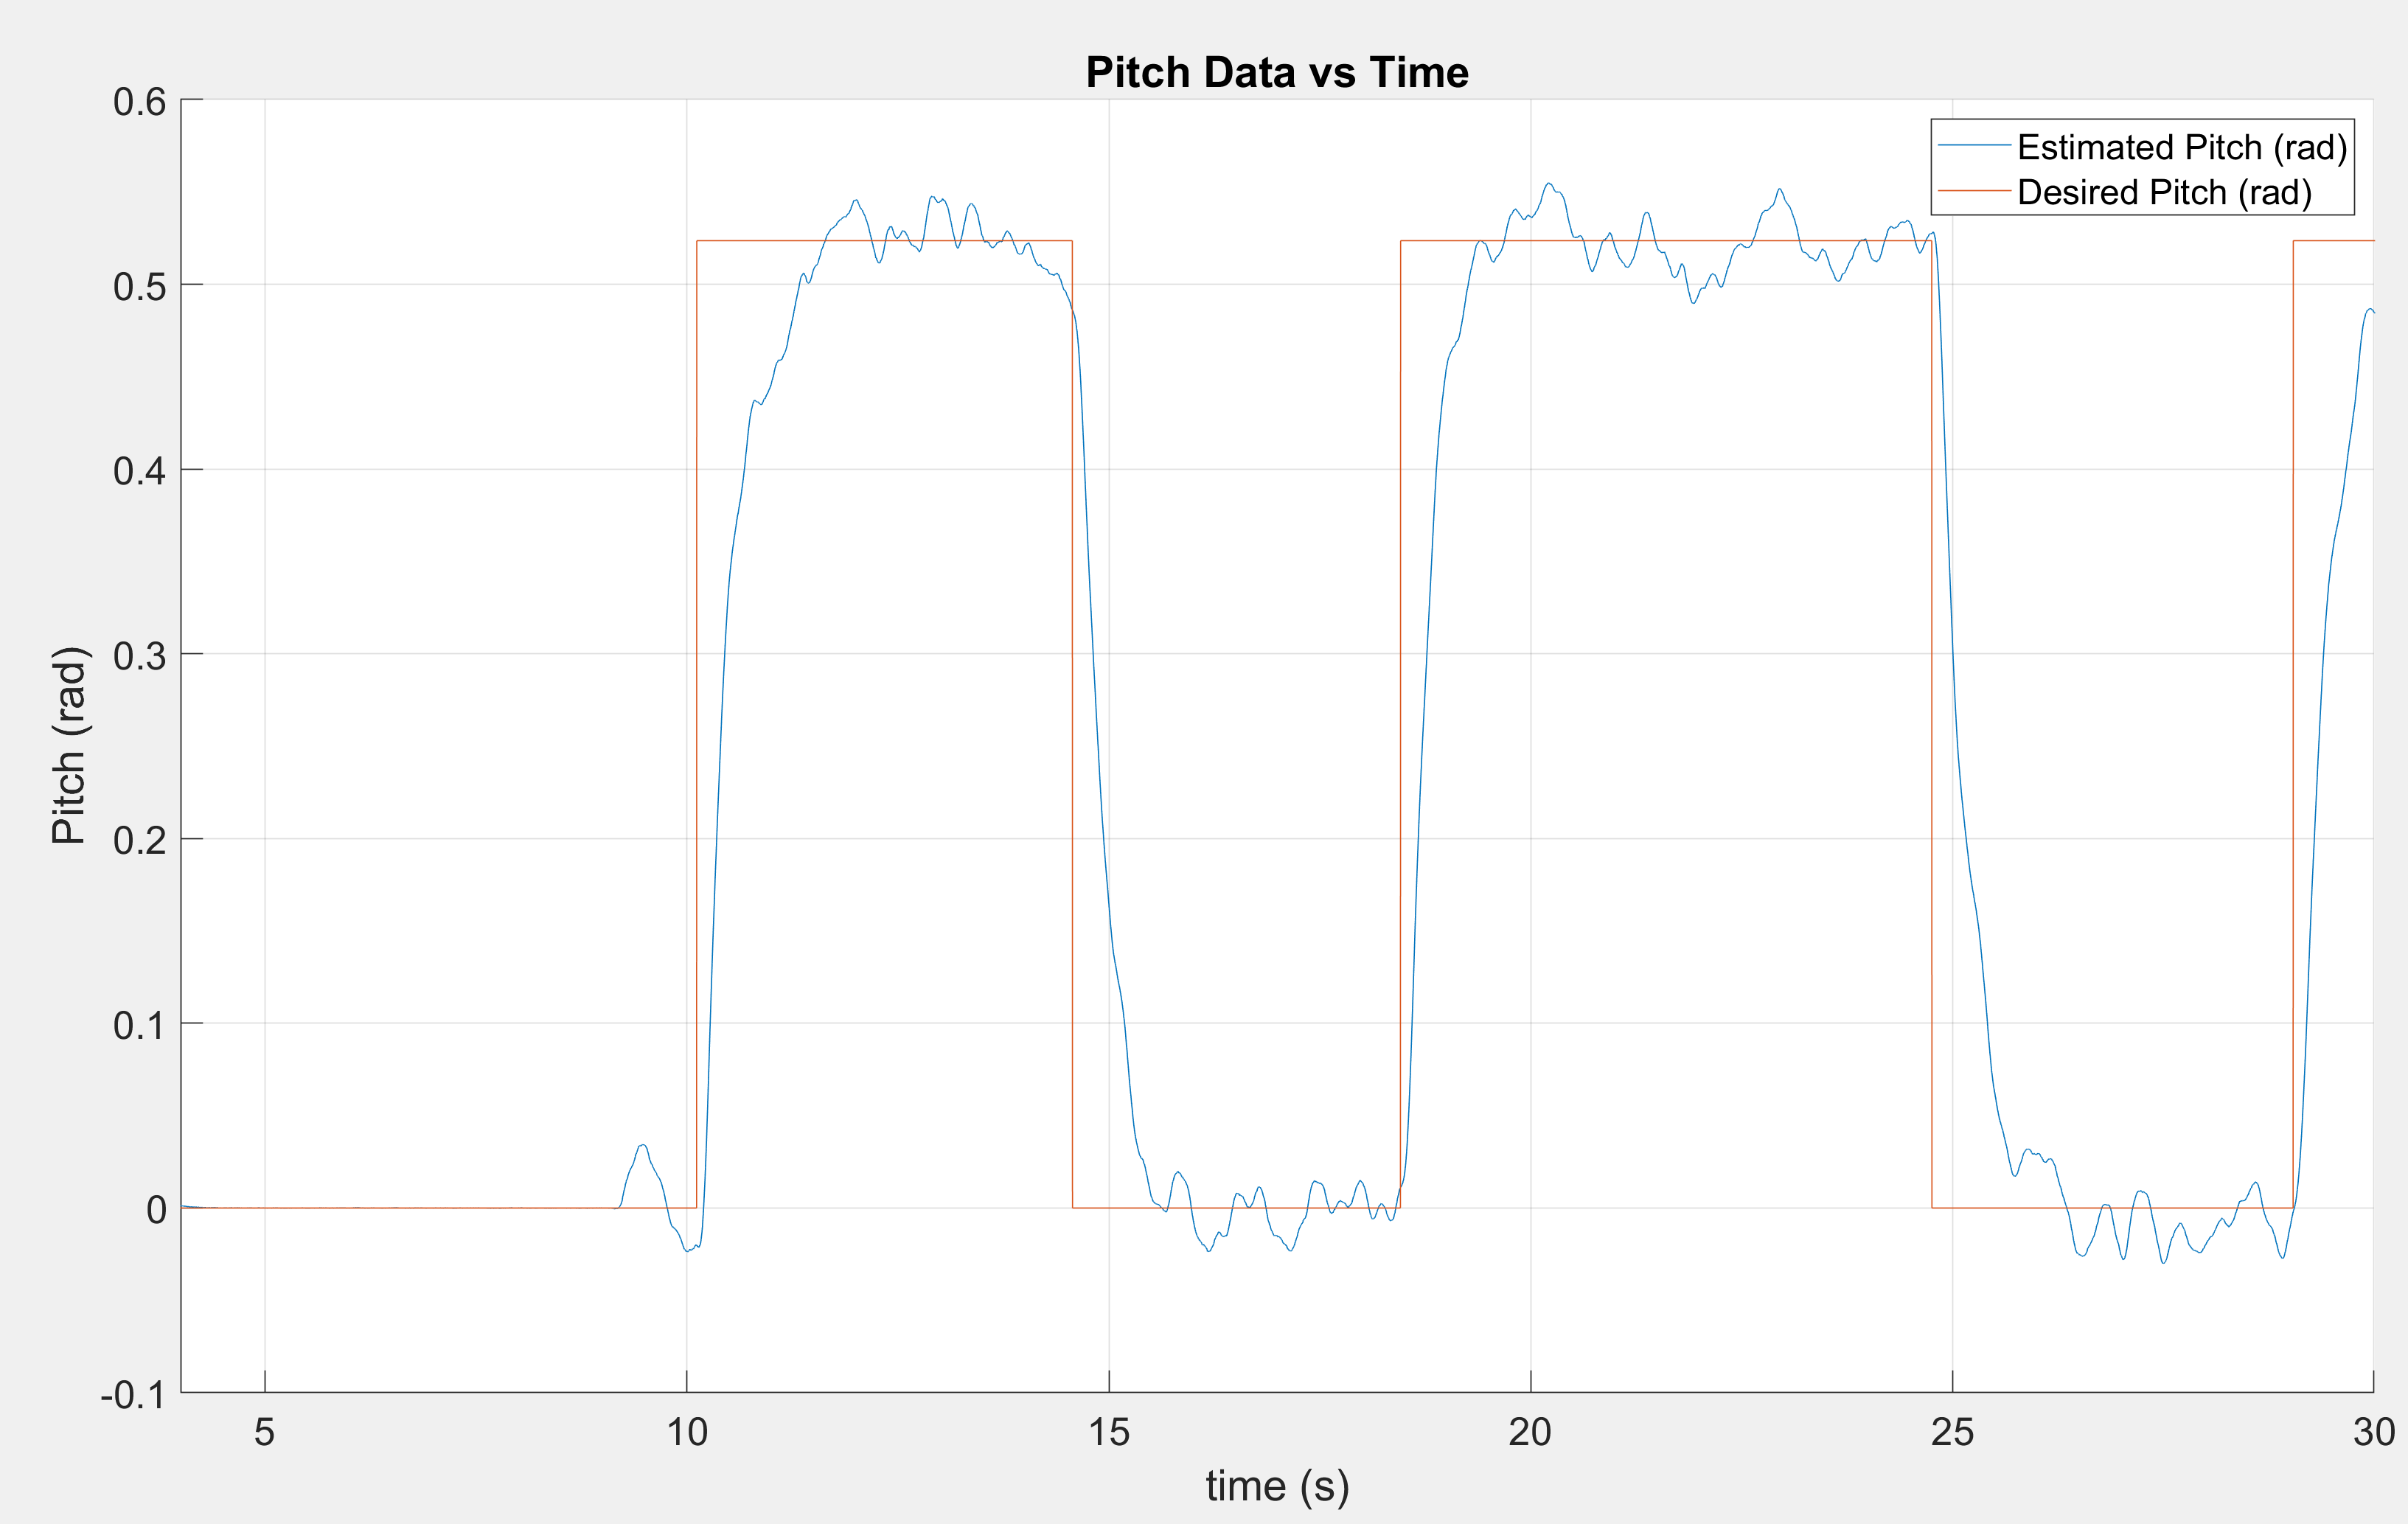
\includegraphics[scale=.19]{4a.png}
\caption{Estimated Pitch and Desired Pitch VS Time}
\end{figure}
\FloatBarrier
\vspace{24pt}

\subsection{Part B}
\begin{figure} [H]
\centering
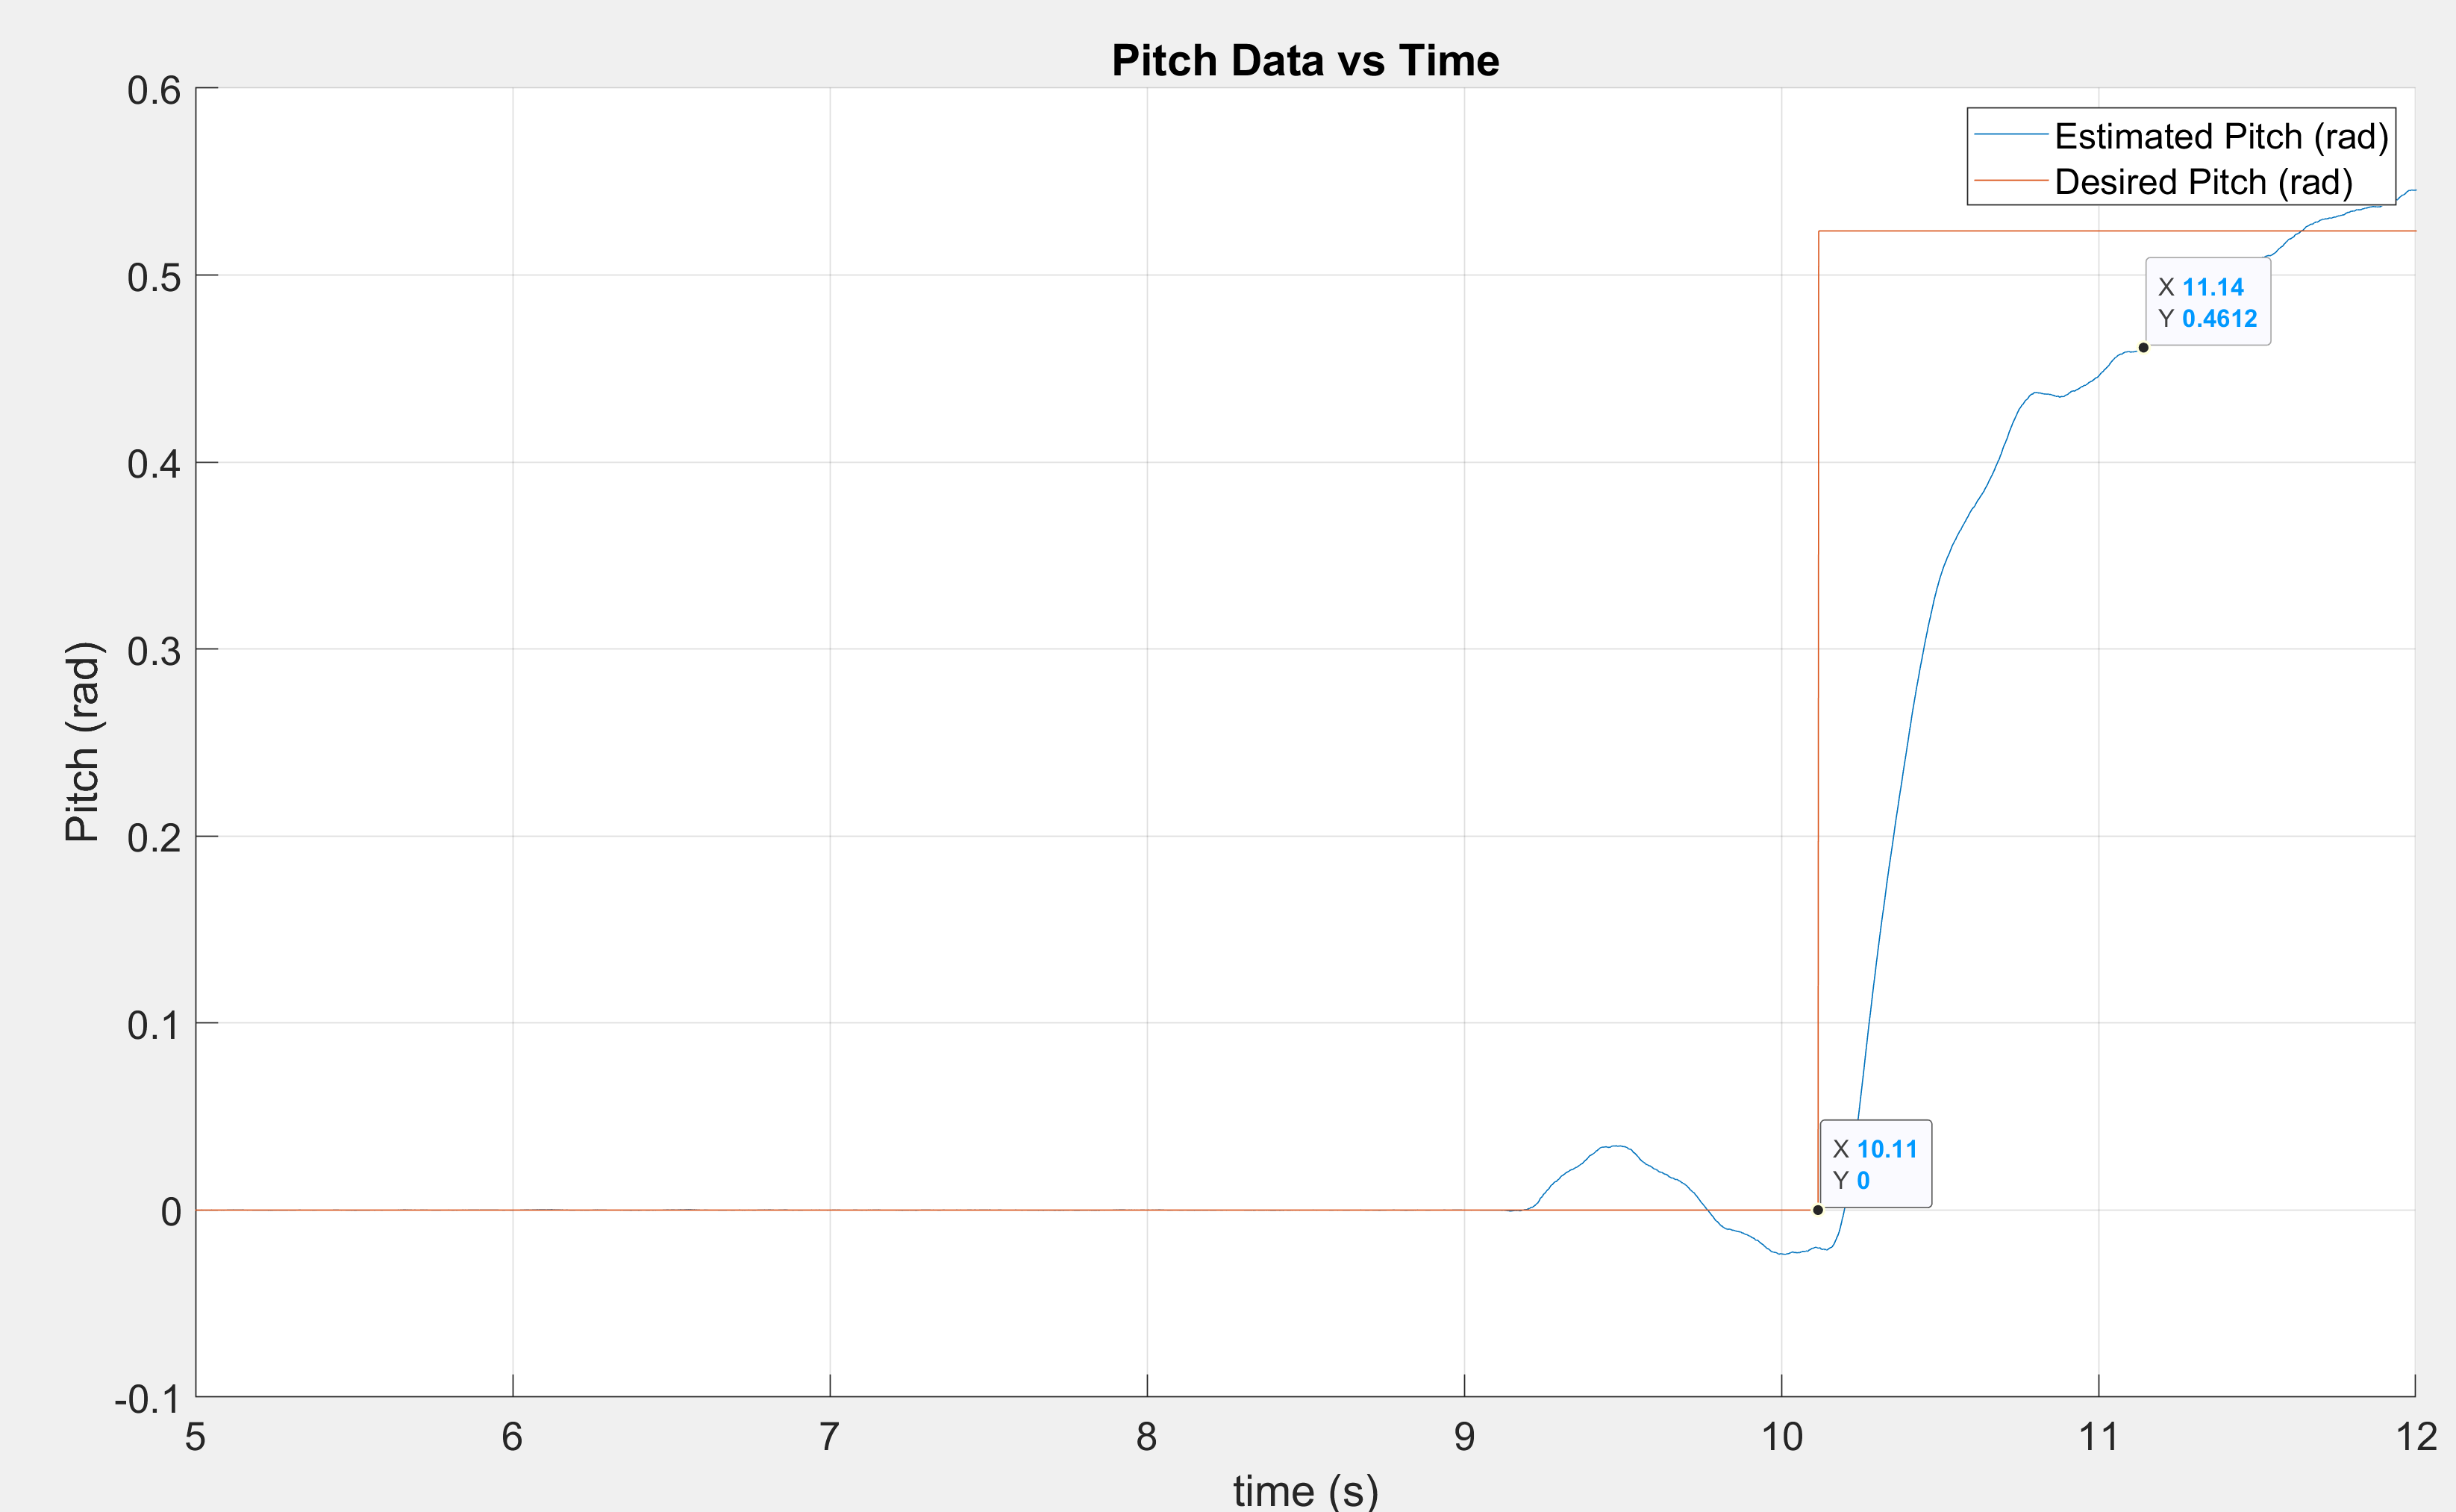
\includegraphics[scale=.19]{ME136Lab4Q4b.png}
\caption{Estimated Pitch and Desired Pitch VS Time (0 to 30 Degrees)}
\end{figure}
\FloatBarrier
\vspace{24pt}
It takes 1.03 seconds for the system to go from 0\% to 90\% of its final value. 


\section{Purposefully Unstable Rates Controller}

\subsection{Part A}
\begin{figure} [H]
\centering
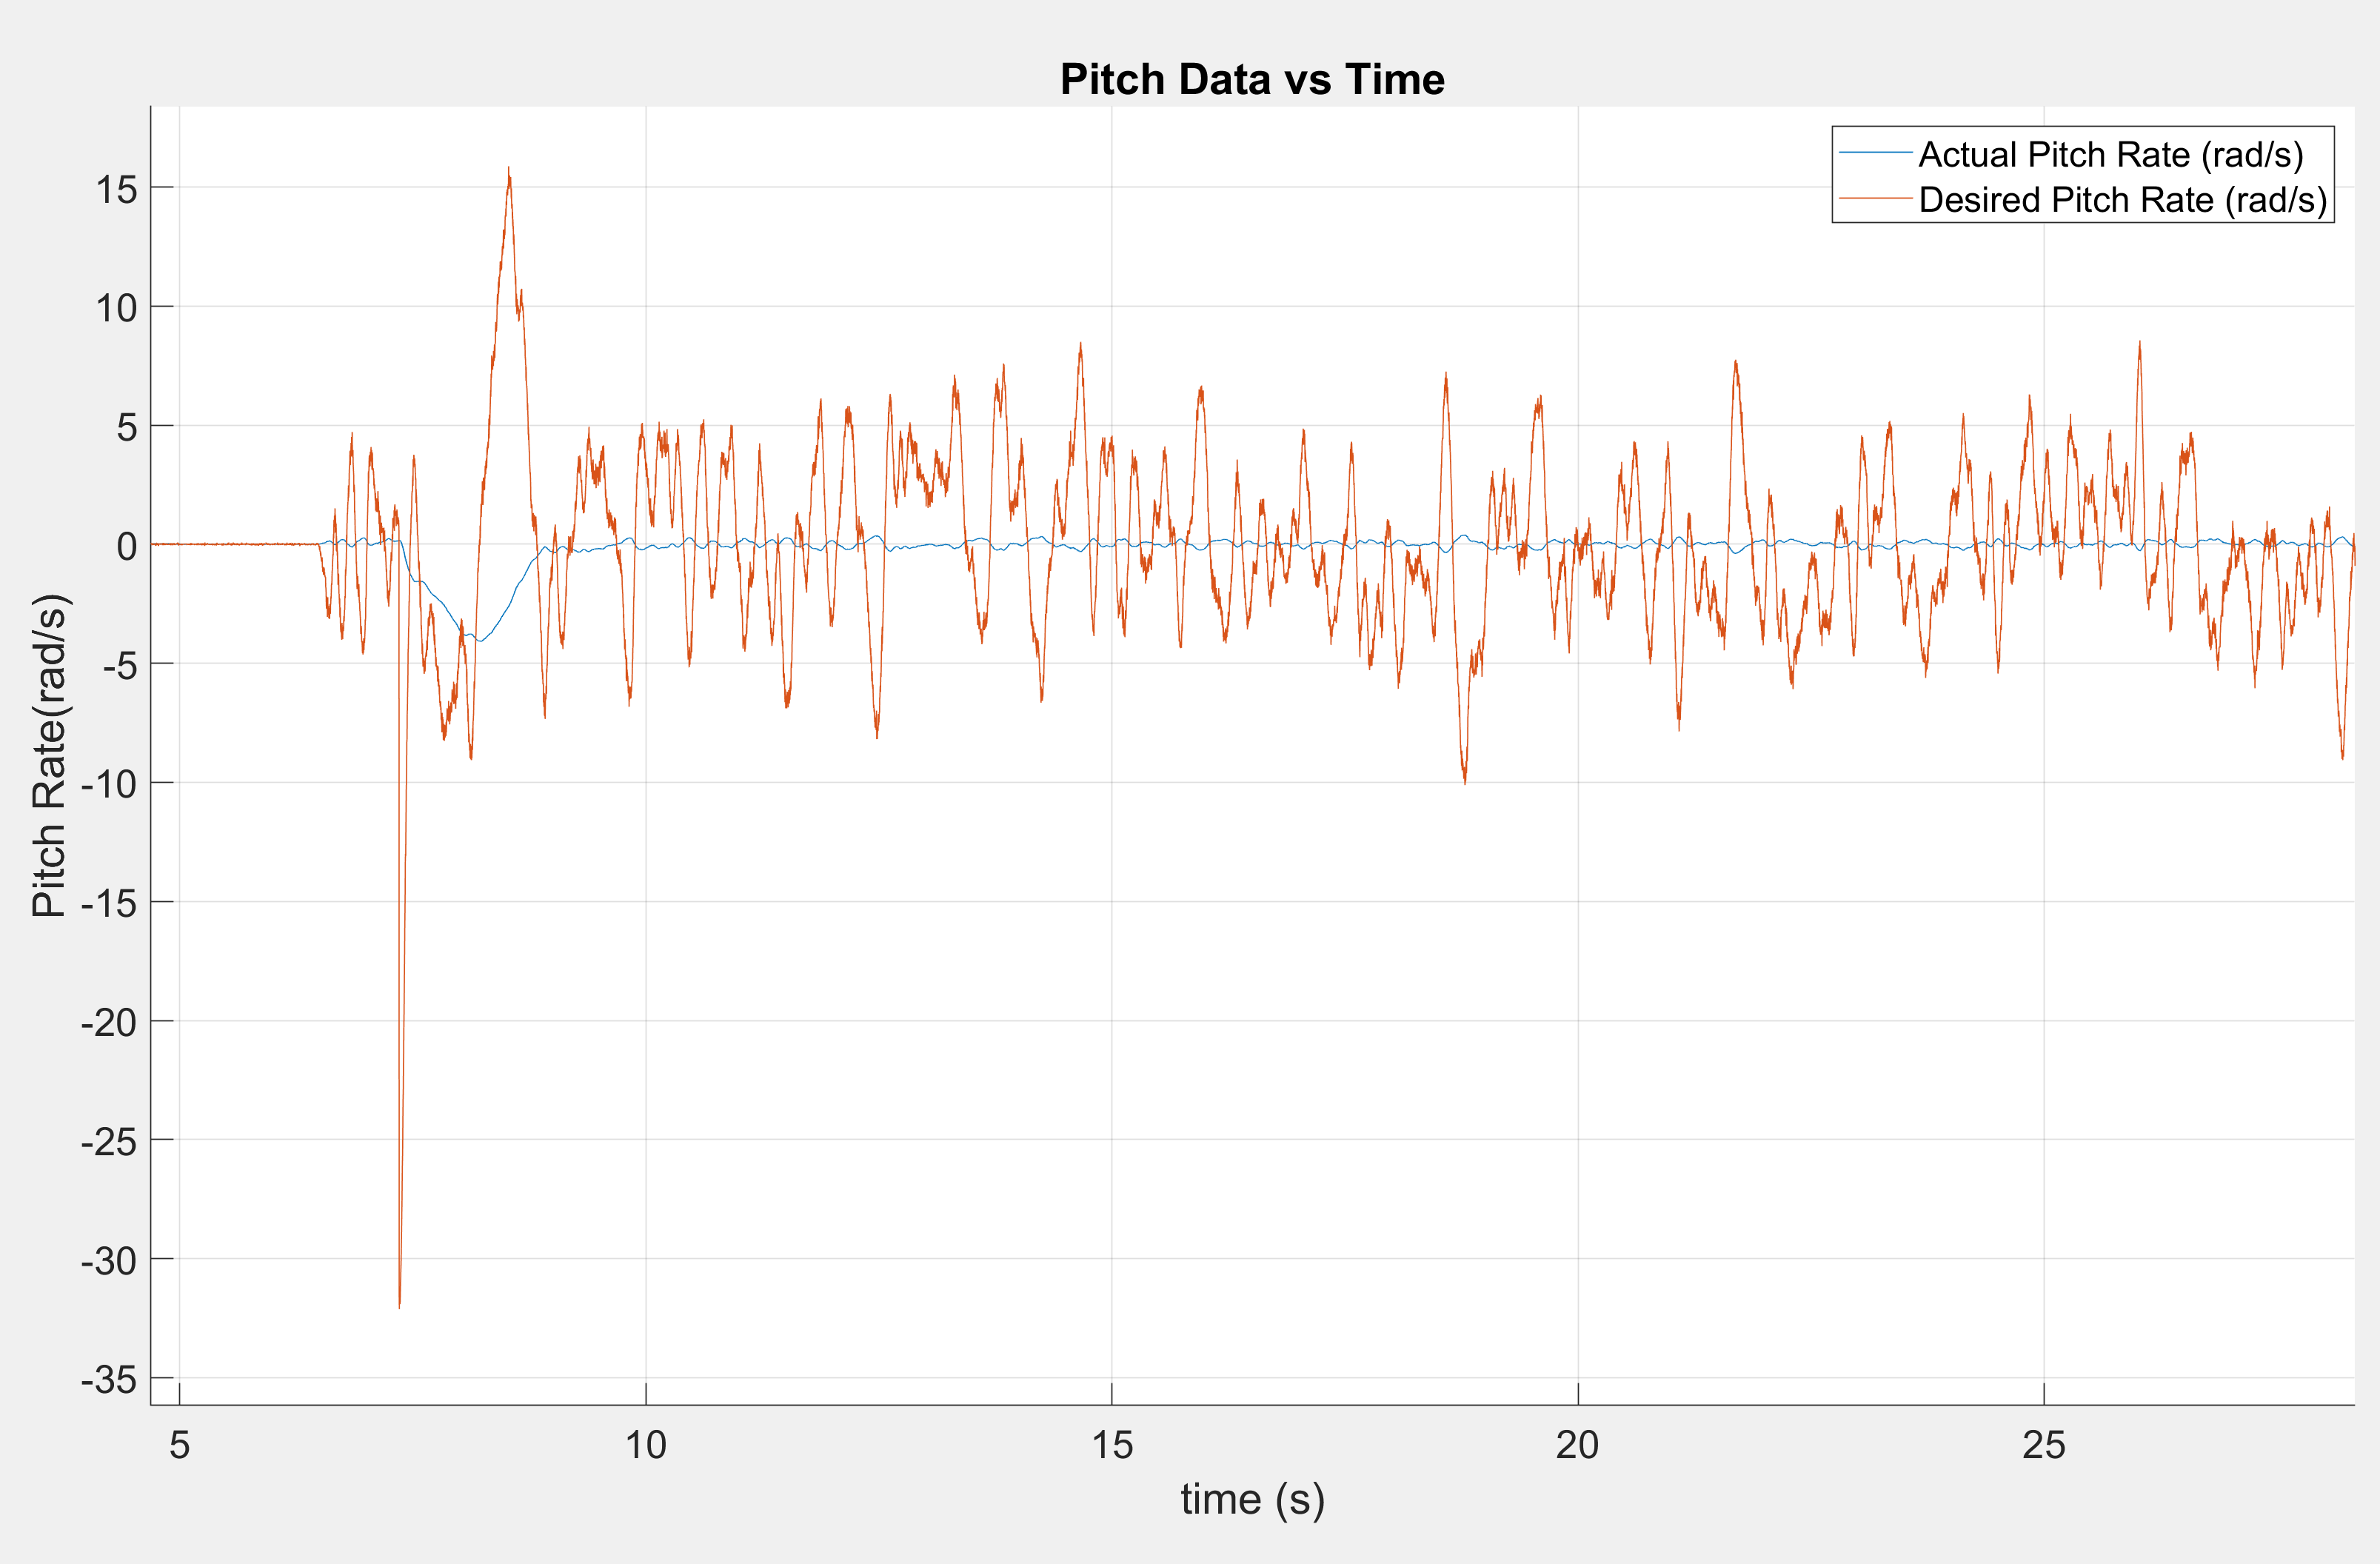
\includegraphics[scale=.19]{ME136Lab4Q5a.png}
\caption{Estimated Pitch Rate and Desired Pitch Rate VS Time}
\end{figure}
\FloatBarrier
\vspace{24pt}

\subsection{Part B}
It takes 22 milliseconds for the angular velocity to double.

\subsection{Part C}
The time-to-double measured in our experiment is much faster than what we would predict. We would predict that the angular velocity would grow as fast as the expected values shown in the plot. However, we know that the controller can correct itself and so it doubles faster than we would expect it to.

\section{Low Thrust Experiments}
\subsection{Part A}
\begin{figure} [H]
\centering
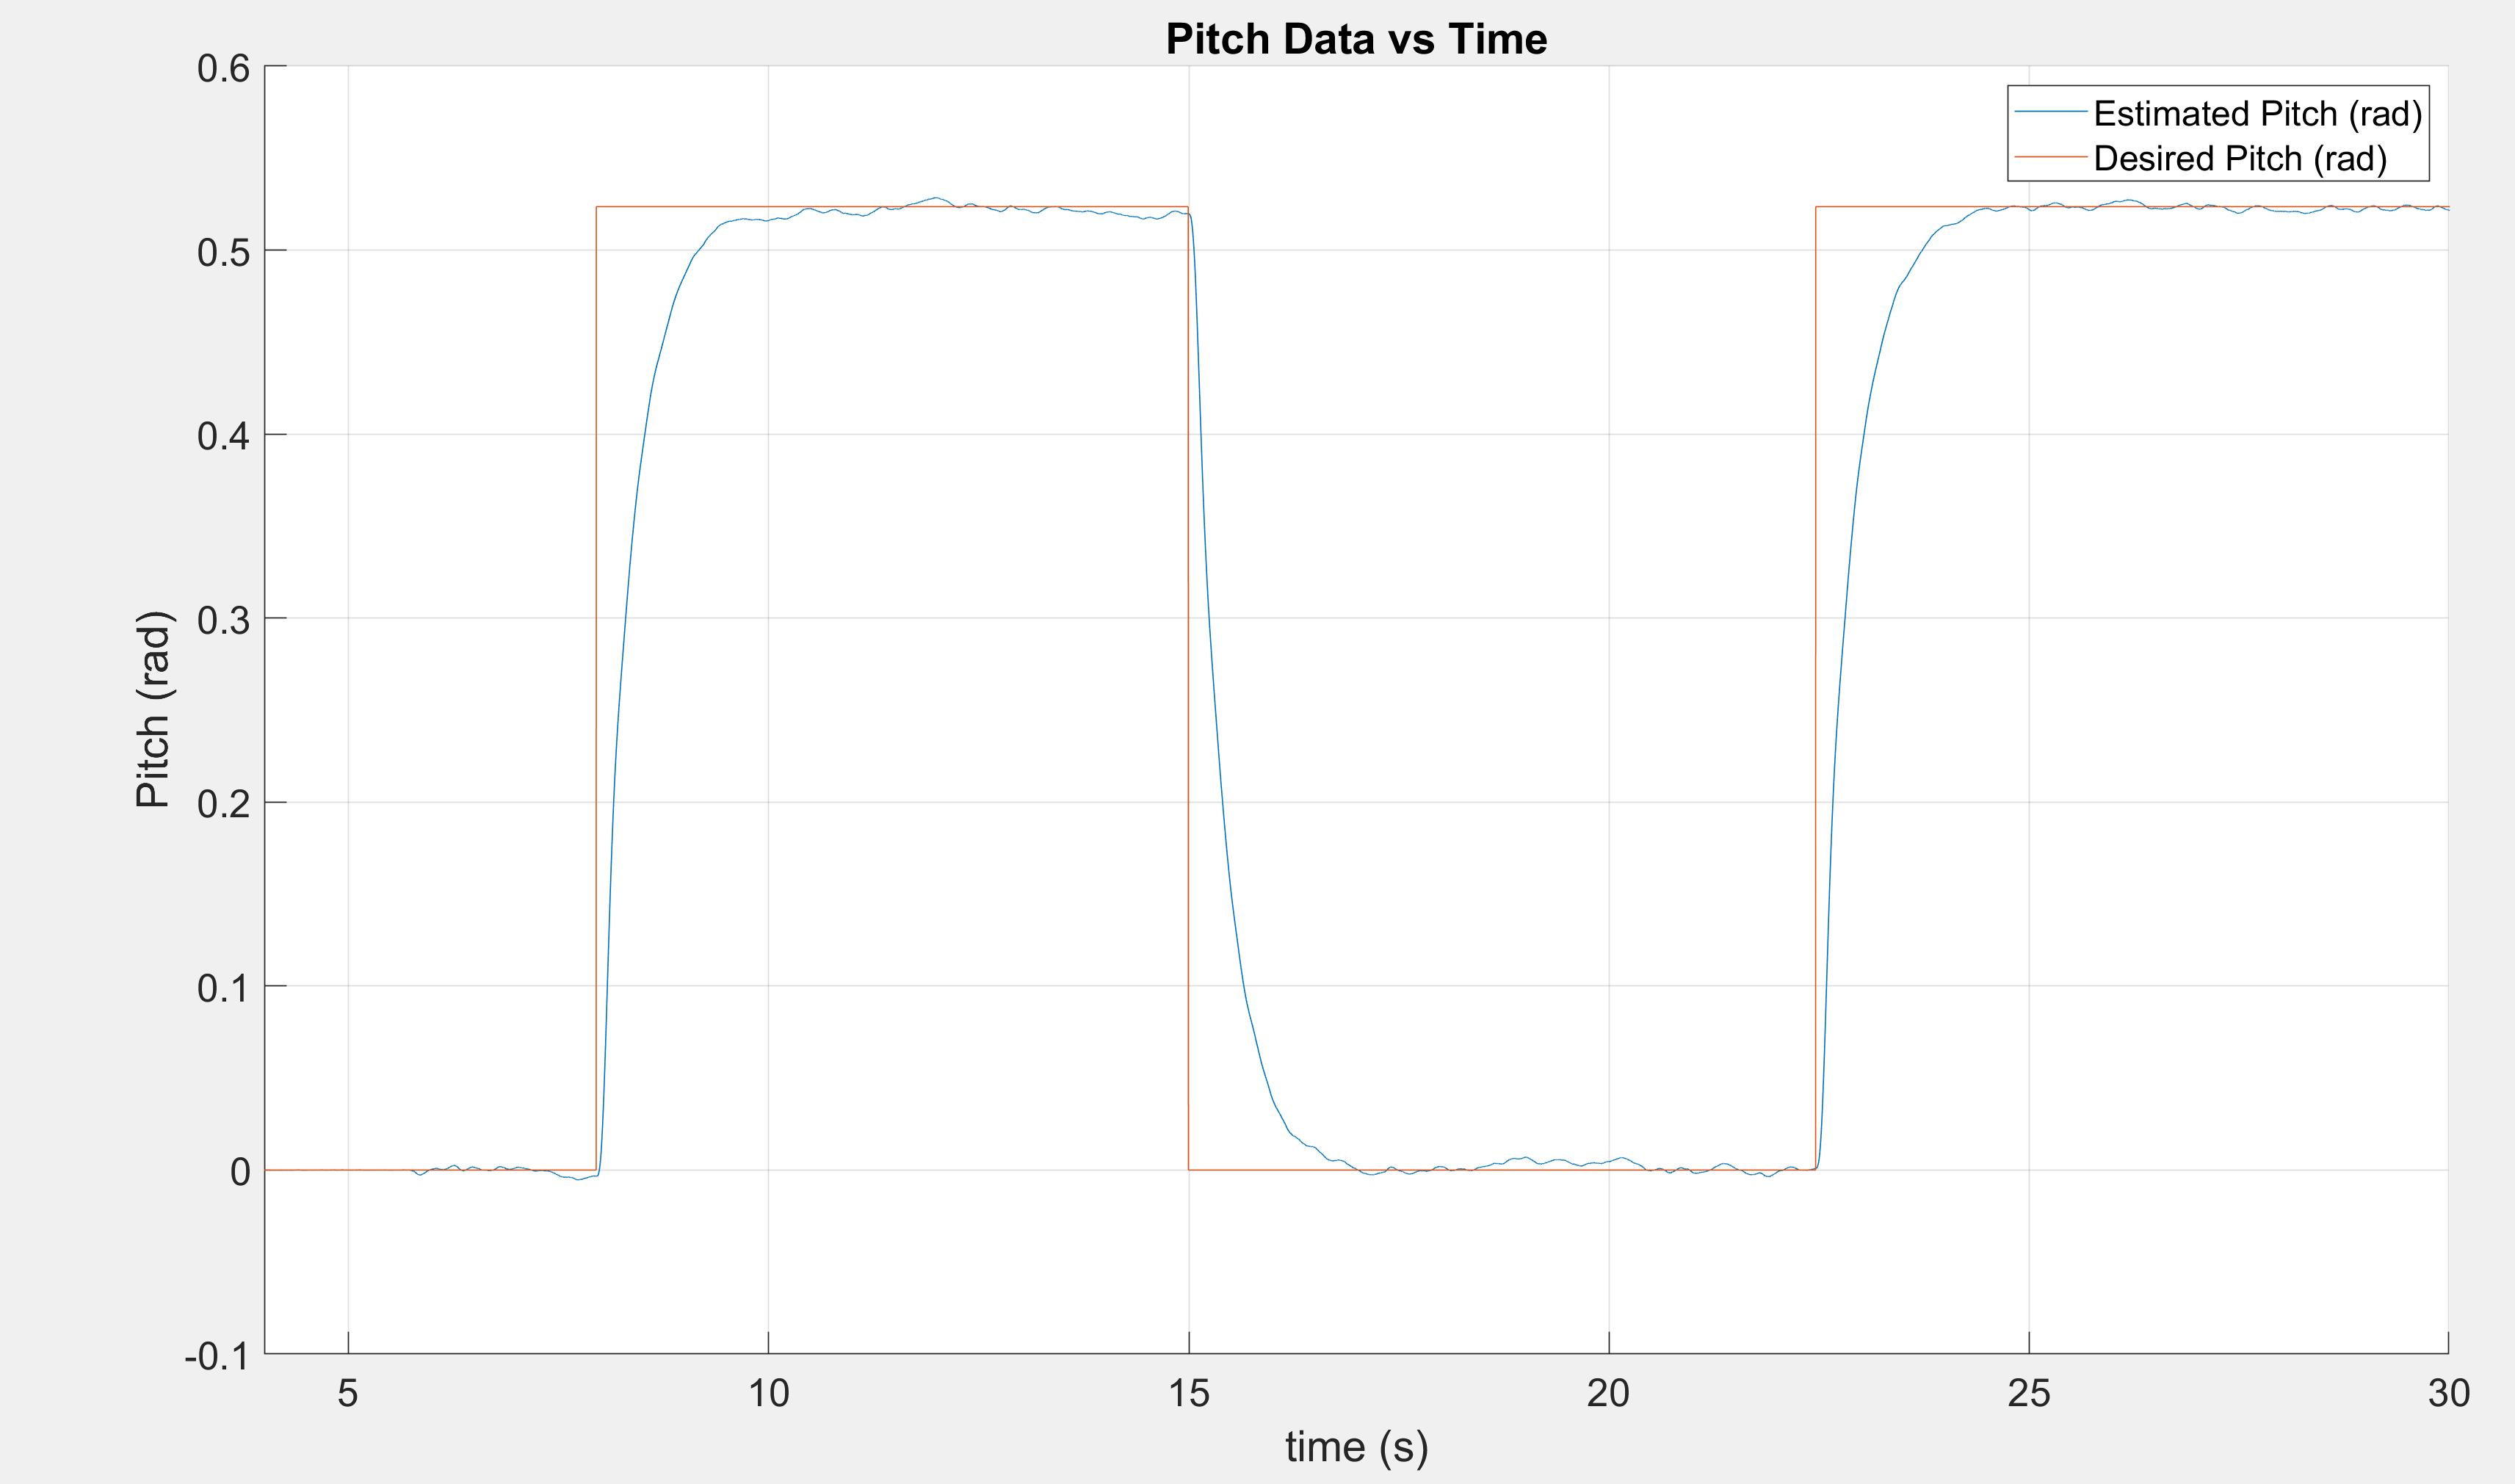
\includegraphics[scale=.19]{ME136Lab4Q6a.png}
\caption{Estimated Pitch and Desired Pitch VS Time}
\end{figure}
\FloatBarrier
\vspace{24pt}

\subsection{Part B}
\begin{figure} [H]
\centering
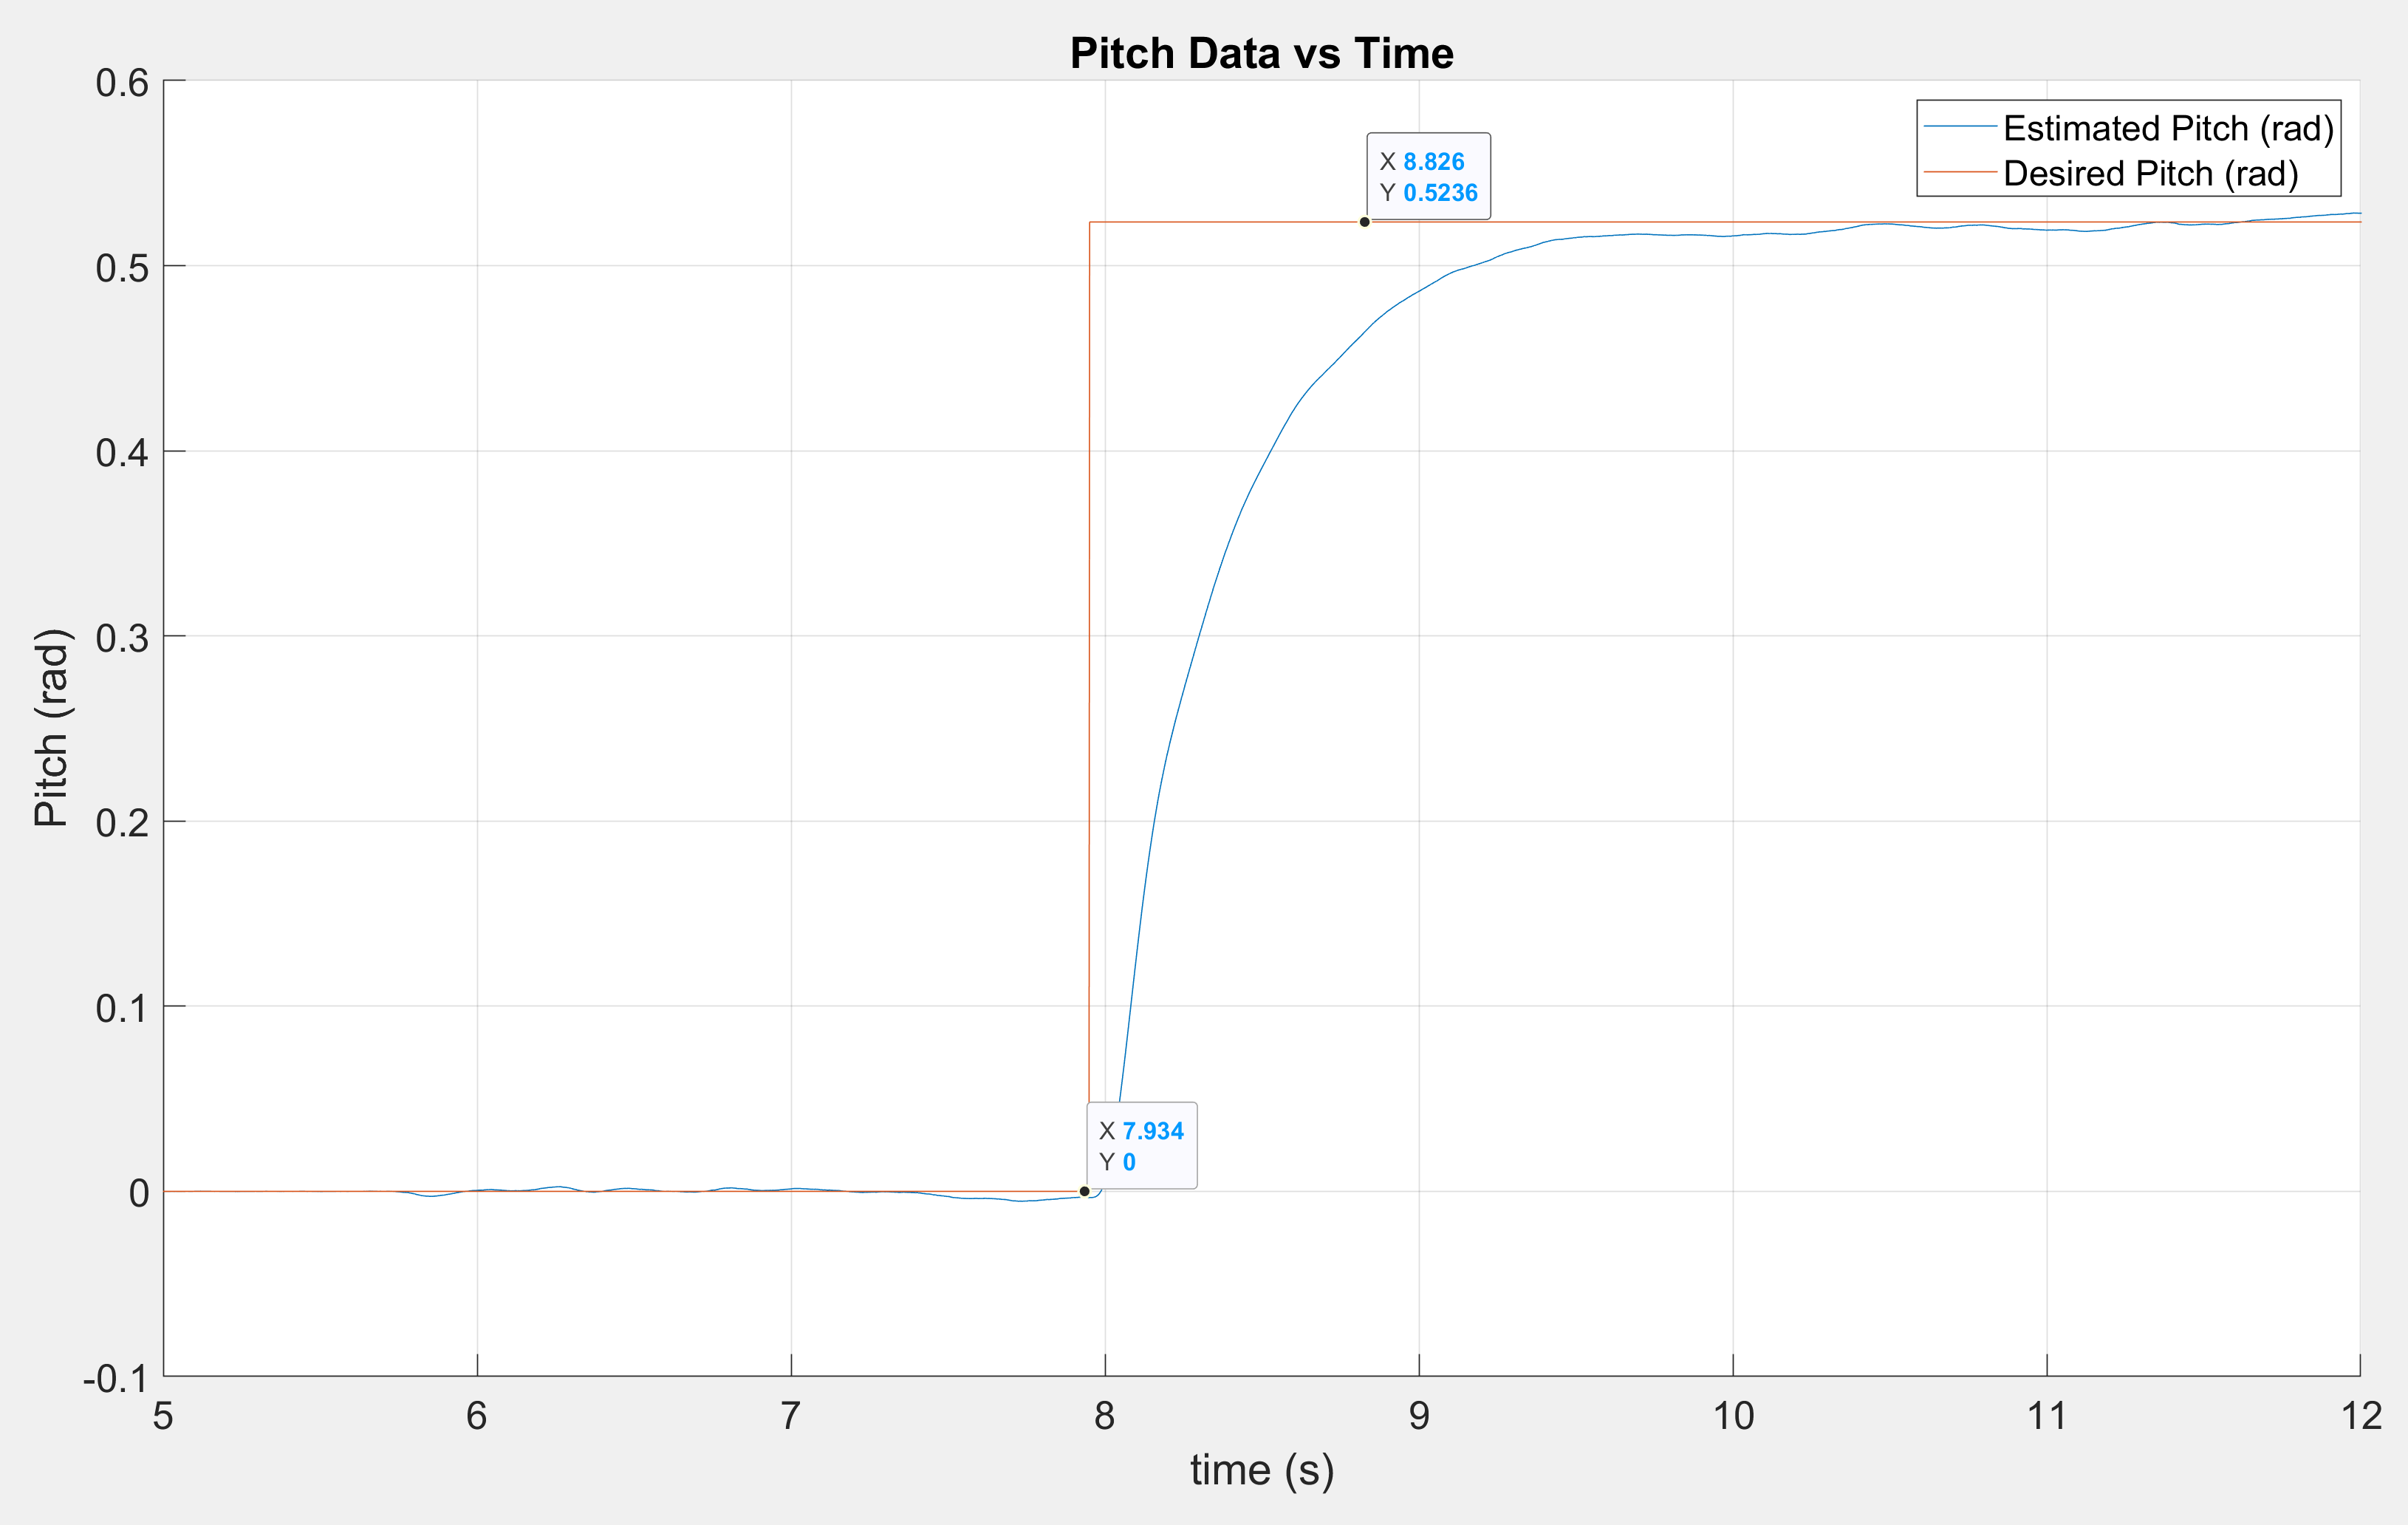
\includegraphics[scale=.19]{ME136Lab4Q6b.png}
\caption{Estimated Pitch and Desired Pitch VS Time (0 to 30 degrees)}
\end{figure}
\FloatBarrier
\vspace{24pt}

The rise time is 0.892 seconds and we have no overshoot recorded in our data.

\subsection{Part C}
\begin{figure} [H]
\centering
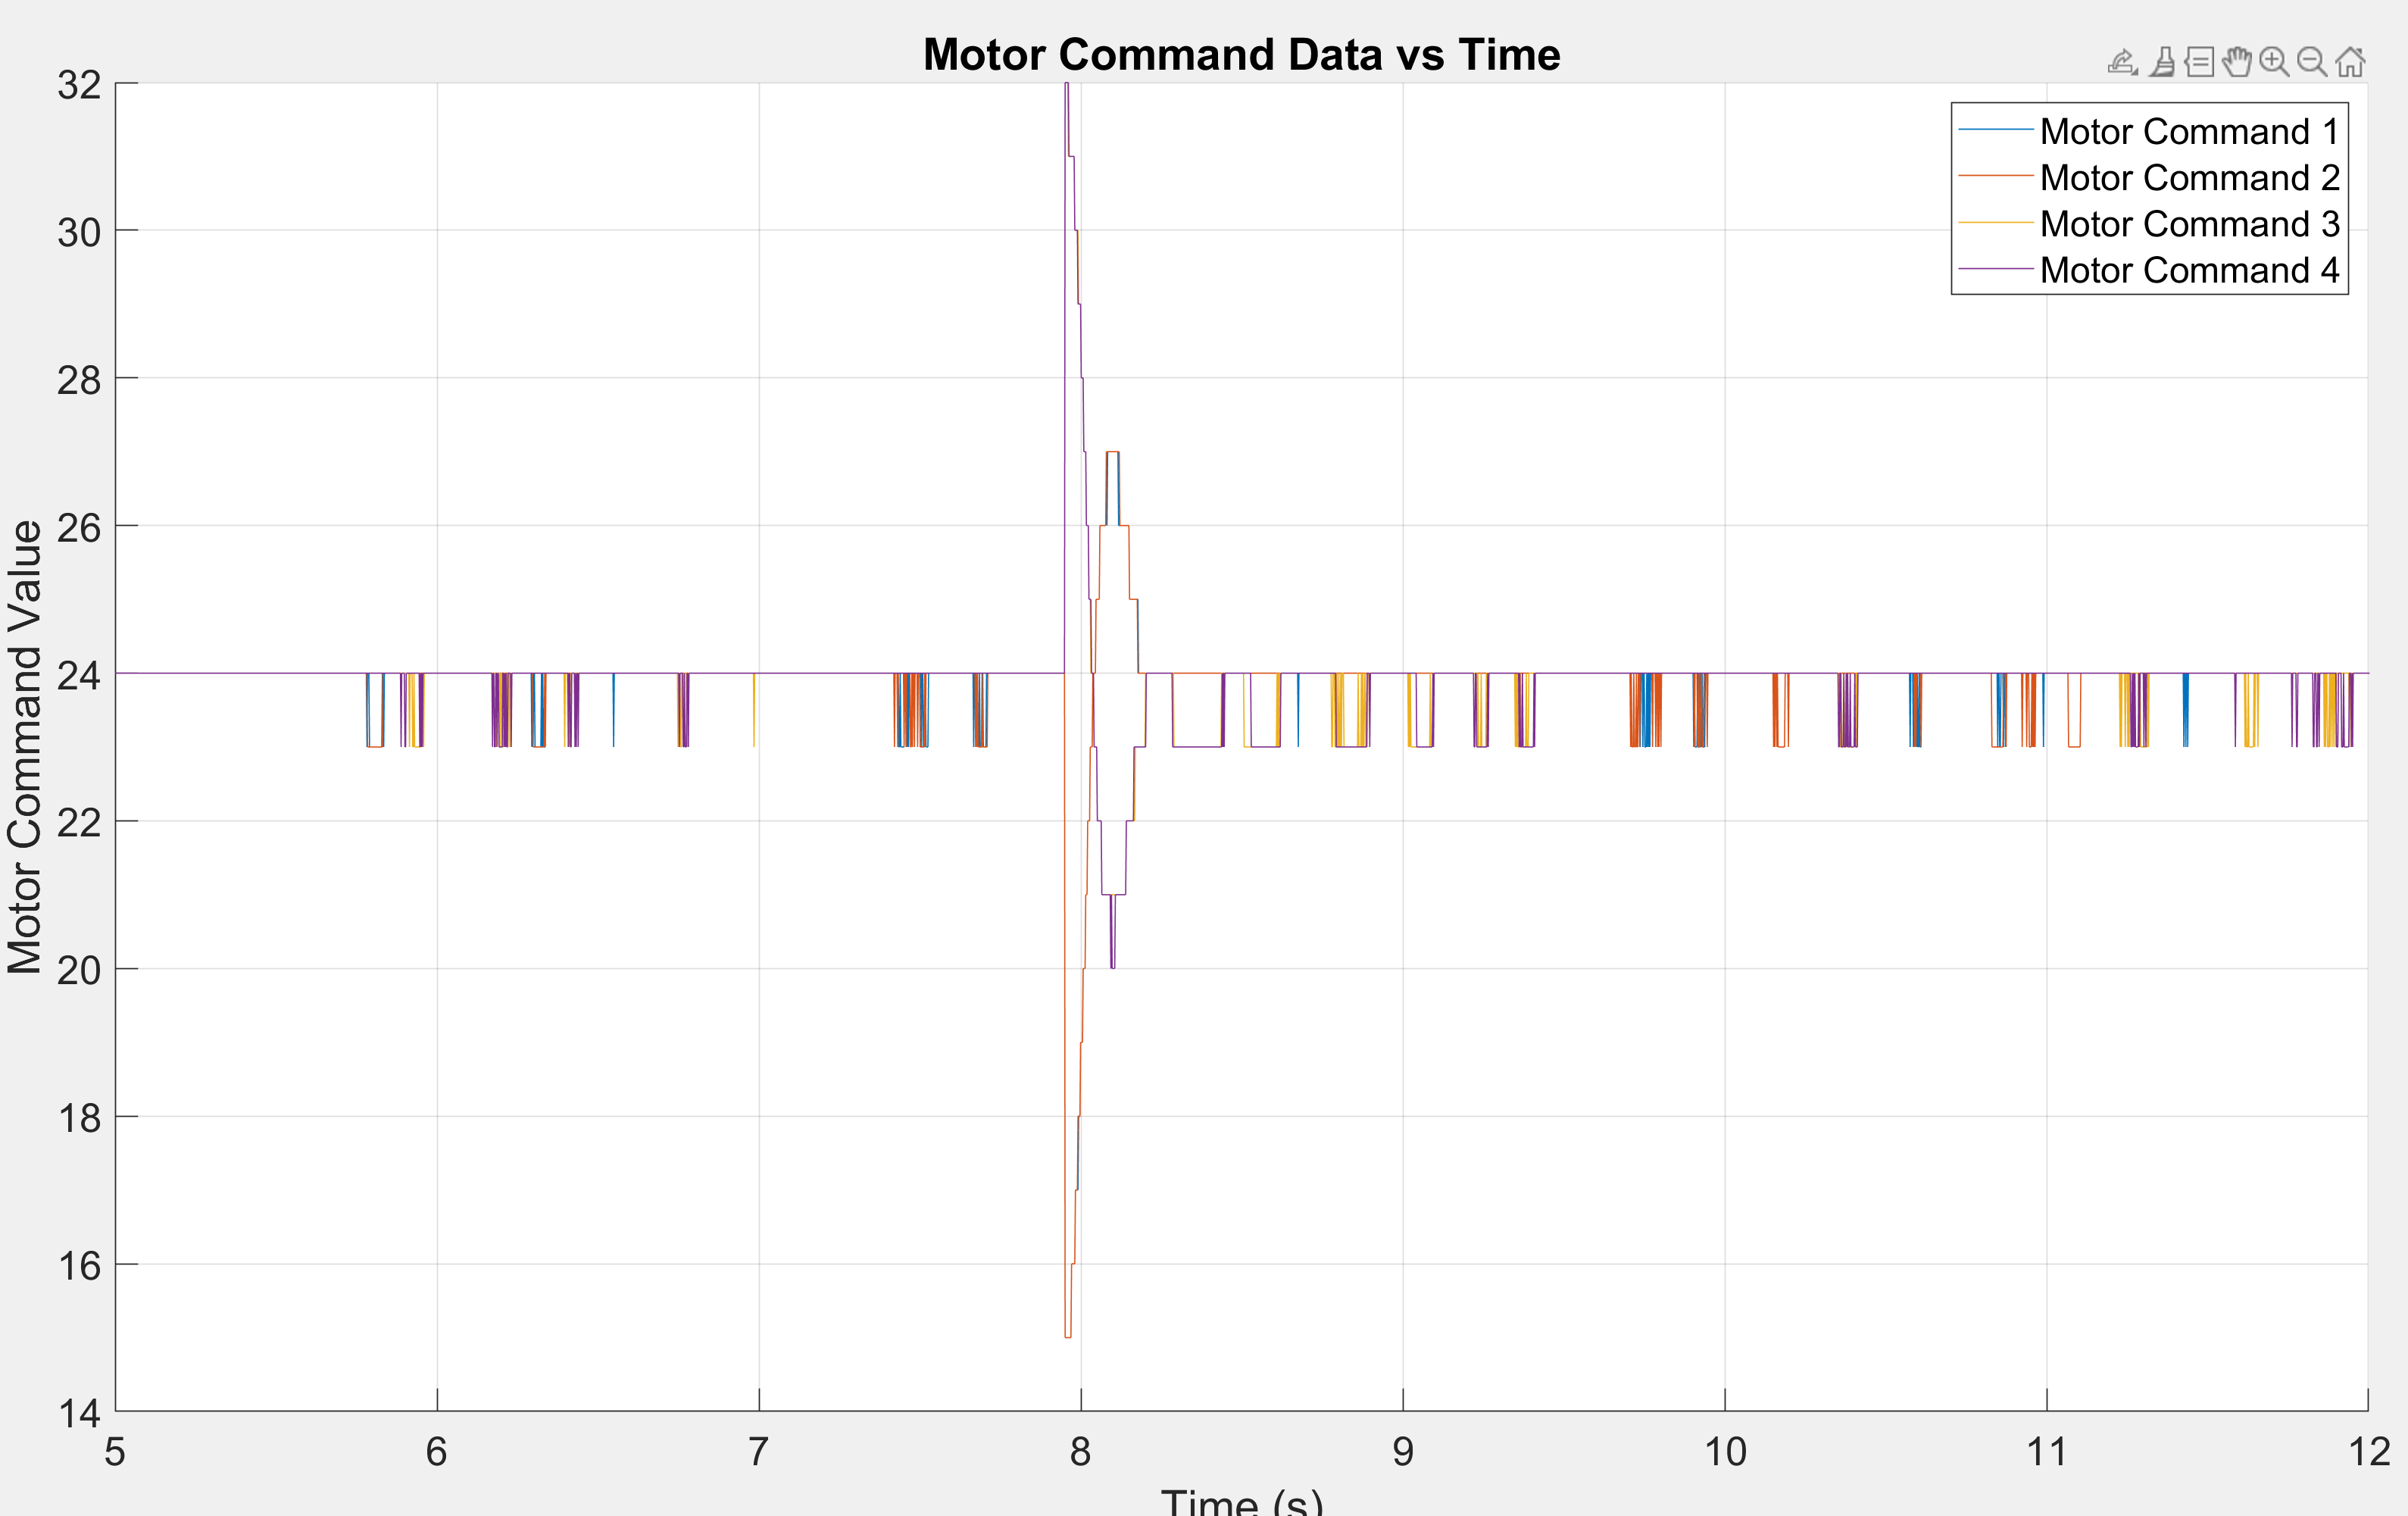
\includegraphics[scale=.19]{ME136Lab4Q6c.png}
\caption{Motor Command Values VS Time}
\end{figure}
\FloatBarrier
\vspace{24pt}

\subsection{Part D}
The response in Part 6 shows a cleaner, smoother curve than the response when we used $8 m/s^2$. The response when using $8 m/s^2$ is very choppy and rises much faster because the acceleration is larger. Both sections are reaching the same endpoint value, however, since the acceleration is larger for the first plot, it rises much quicker and creates a choppier curve while the smaller acceleration rises slower and can gently center once it reaches the correct pitch.

\section{Accidentally Unstable Control}
\subsection{Part A}
\begin{figure} [H]
\centering
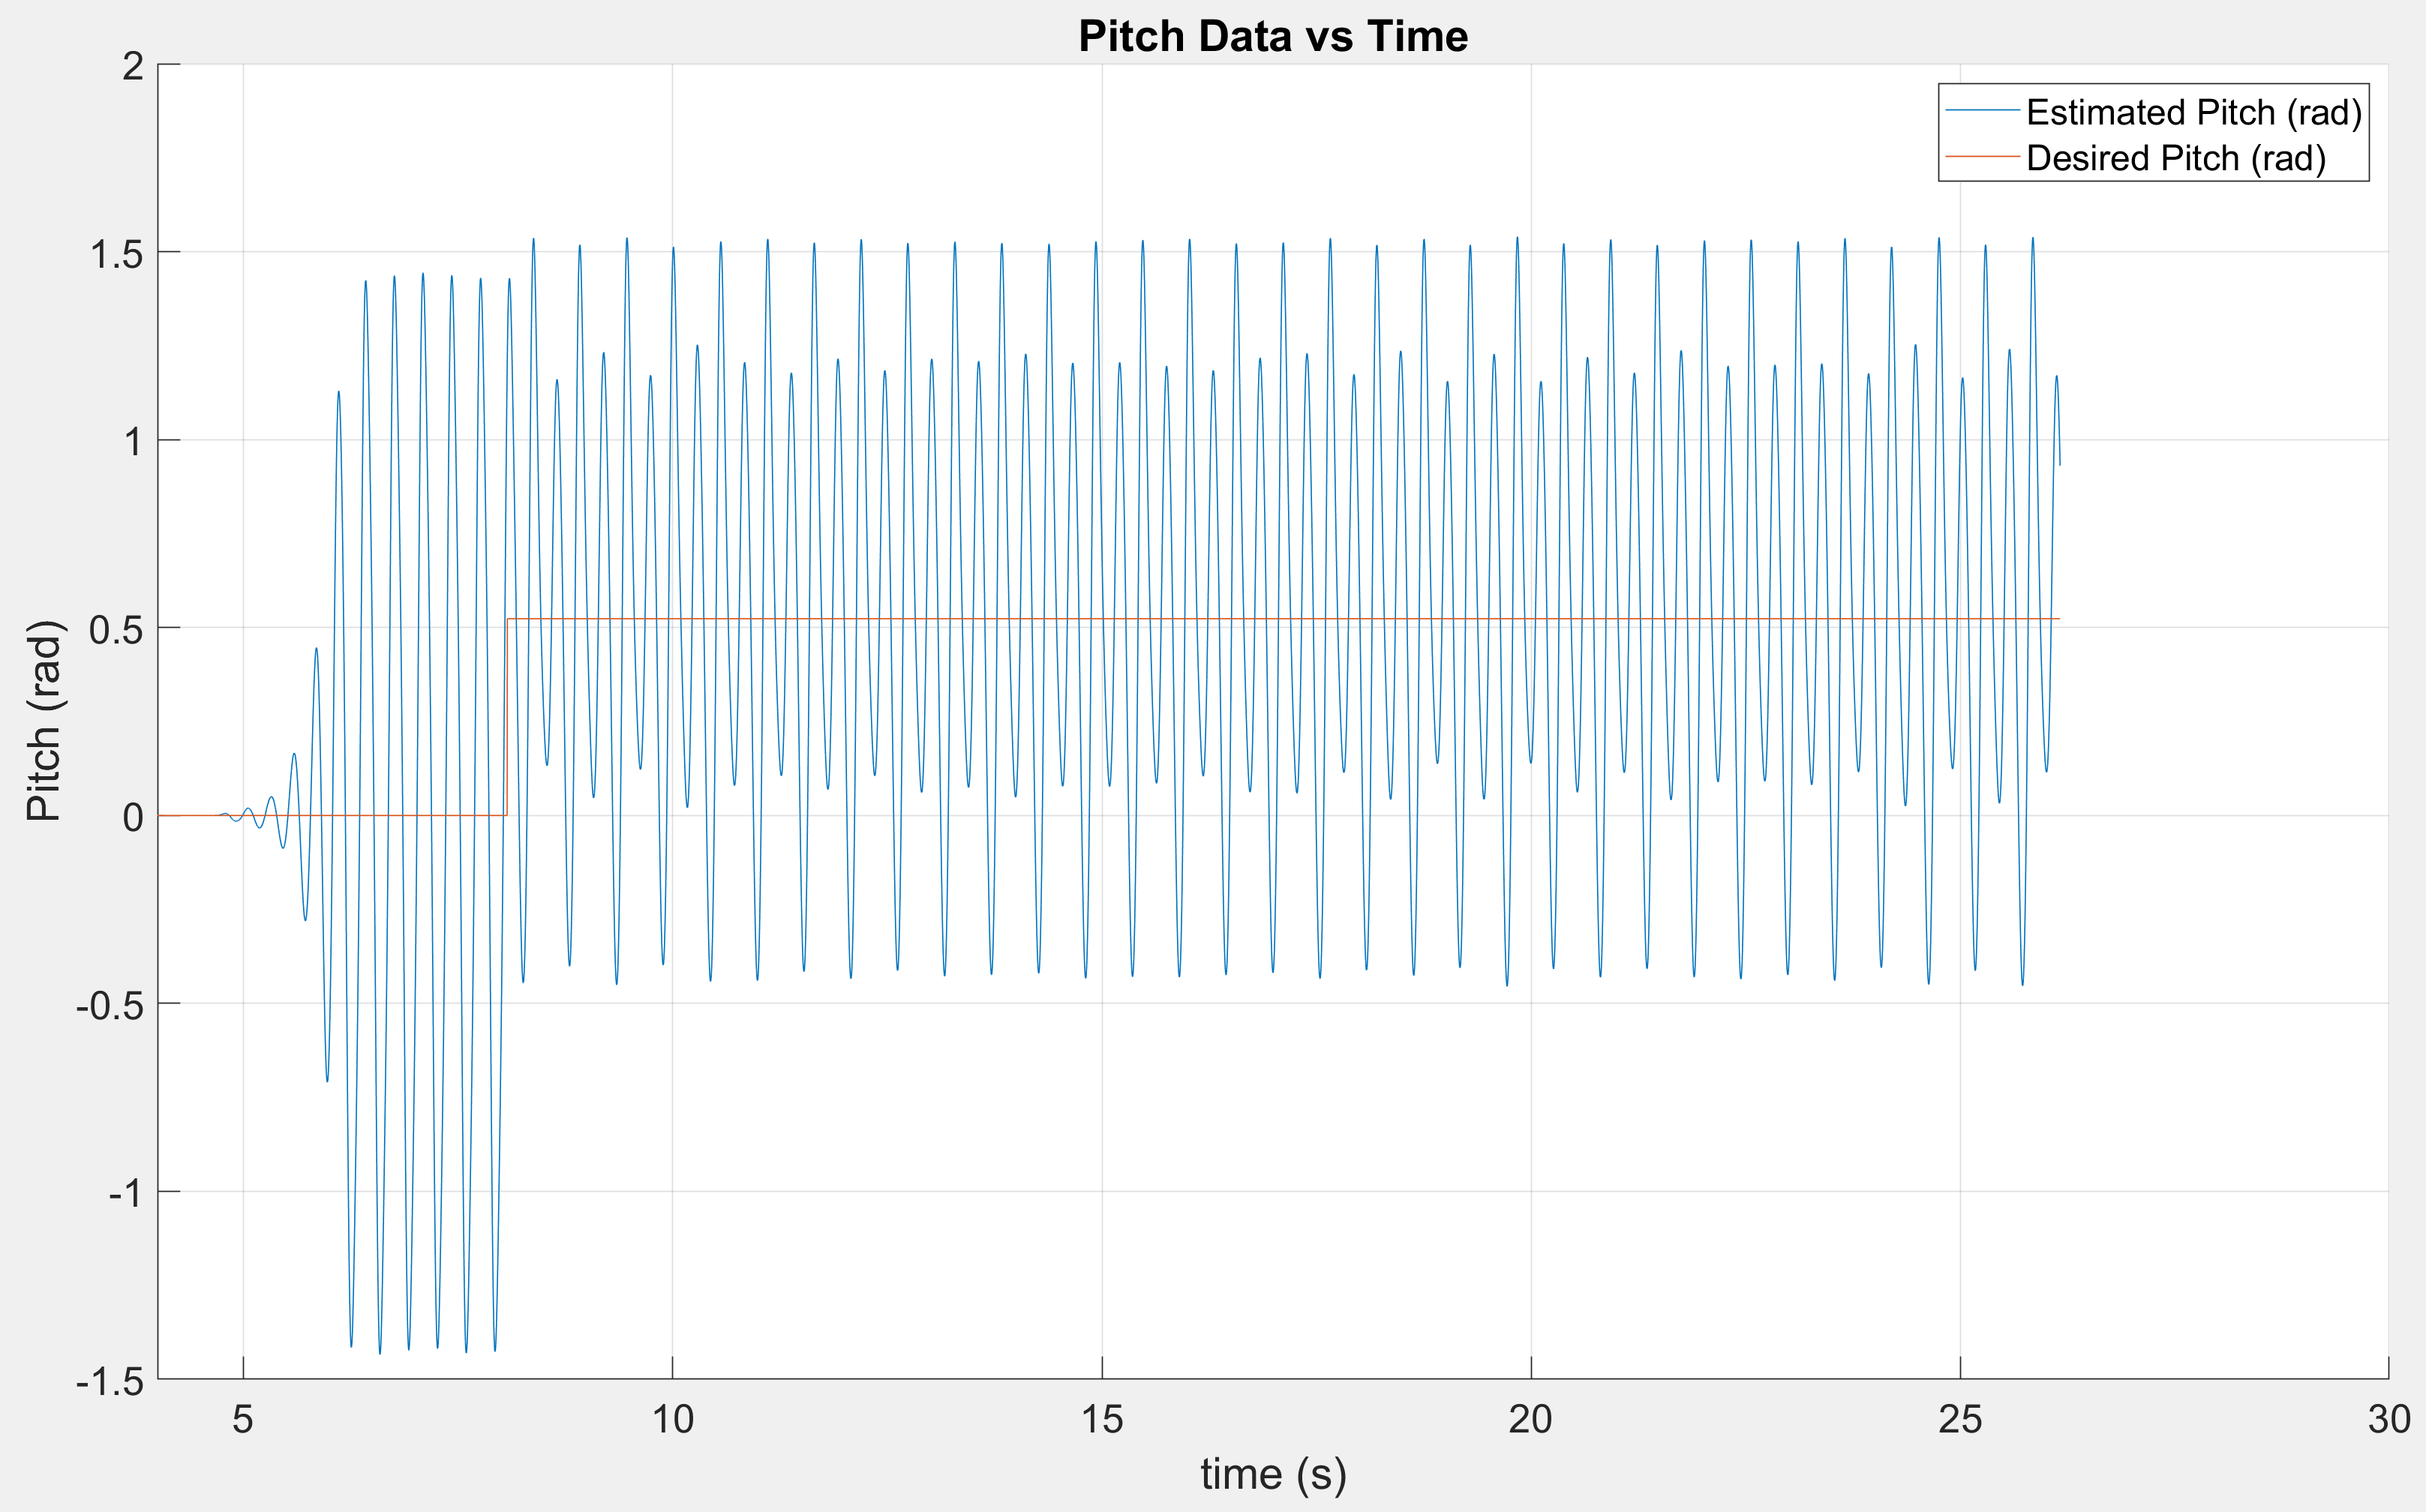
\includegraphics[scale=.19]{ME136Lab4Q7a.png}
\caption{Estimated Pitch and Desired Pitch VS Time}
\end{figure}
\FloatBarrier
\vspace{12pt}

\subsection{Part B}
The instability occurred when the time constant was 0.025s. This value was found by running the simulation at different time constants, and if the rotation of the drone was stable, the time constant was halved again. A possible reason why such a small time constant makes the system unstable is due to the calculation of the estimated pitch at such small increments that the motor control is unable to account for the changes. Due to the small time constant, the changes in the estimated pitch are over-corrected and this cycle continues on. The lesson that we took away is that our control system does not have fine enough control to run on such a small time constant and that if you need a system to run like this, it needs to be better characterized and have finer control.

\subsection{Part C}
Since we were doing this experiment in a simulation, there was no friction that was acting on the drone. However, friction would likely make the system less prone to instability since the force being outputted by the motors would have a weakened effect, allowing for smoother motion in the drone. This would get rid of some of the issues in the overshoot caused by the repeated quick calculations in the necessary thrust required to get the drone to reach the desired pitch.

\subsection{Part D}
This instability varies from the one that was purposefully triggered in that the drone is unable to reach an equilibrium. In this case, while the pattern of the pitch is repeatable, the drone did not reach a stable stopping point.

\section{MainLoop Function}

\subsection{Virtual Machine Code}

On the page below is the full listing of our UserCode with comments where we added code to the MainLoop function for lab 4 starting at line 66 with our variables defined in lines 36-41:
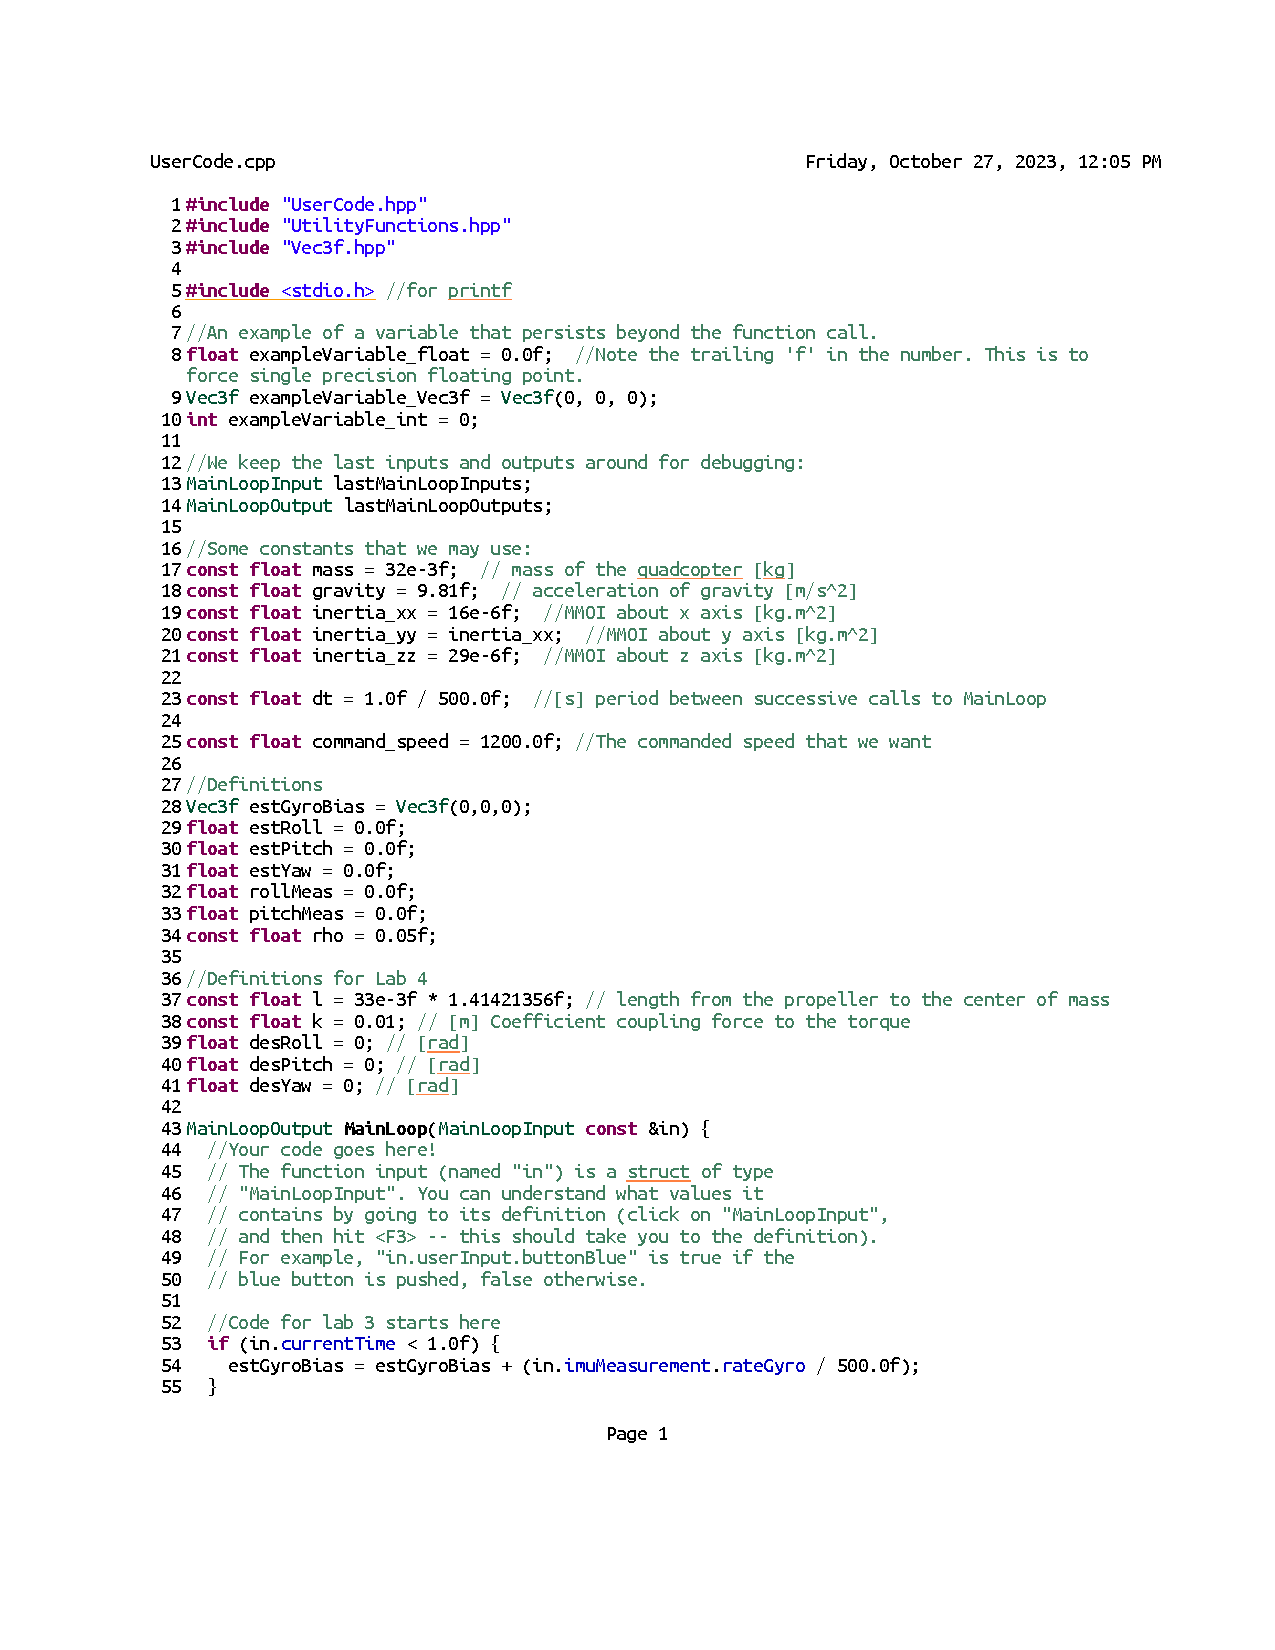
\includepdf[pages=-]{Lab4UserCode.pdf}

On the page below is the full listing of our UtilityCode with comments:
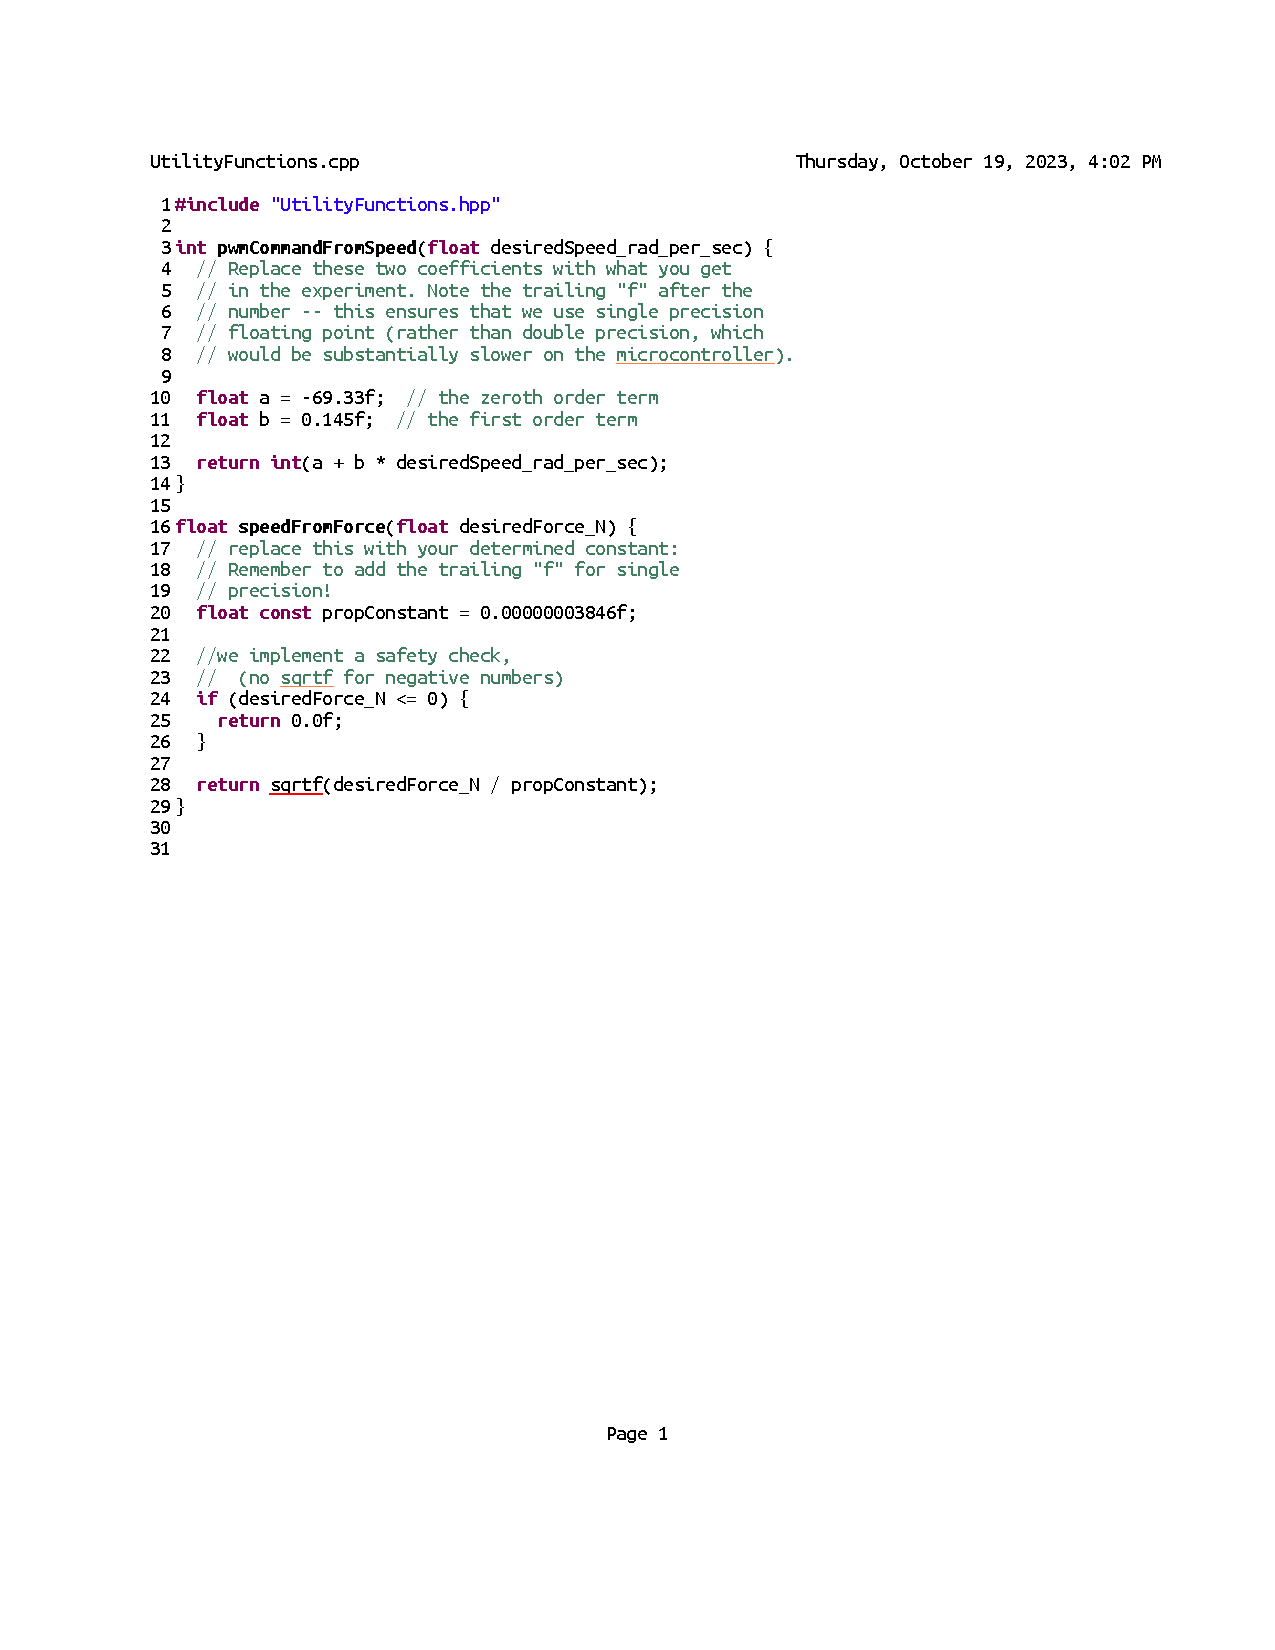
\includepdf[pages=-]{Lab4UtilityCode.pdf}

\subsection{Matlab Code} 
On the page below is our Matlab code we used for the plots of our deliverables.

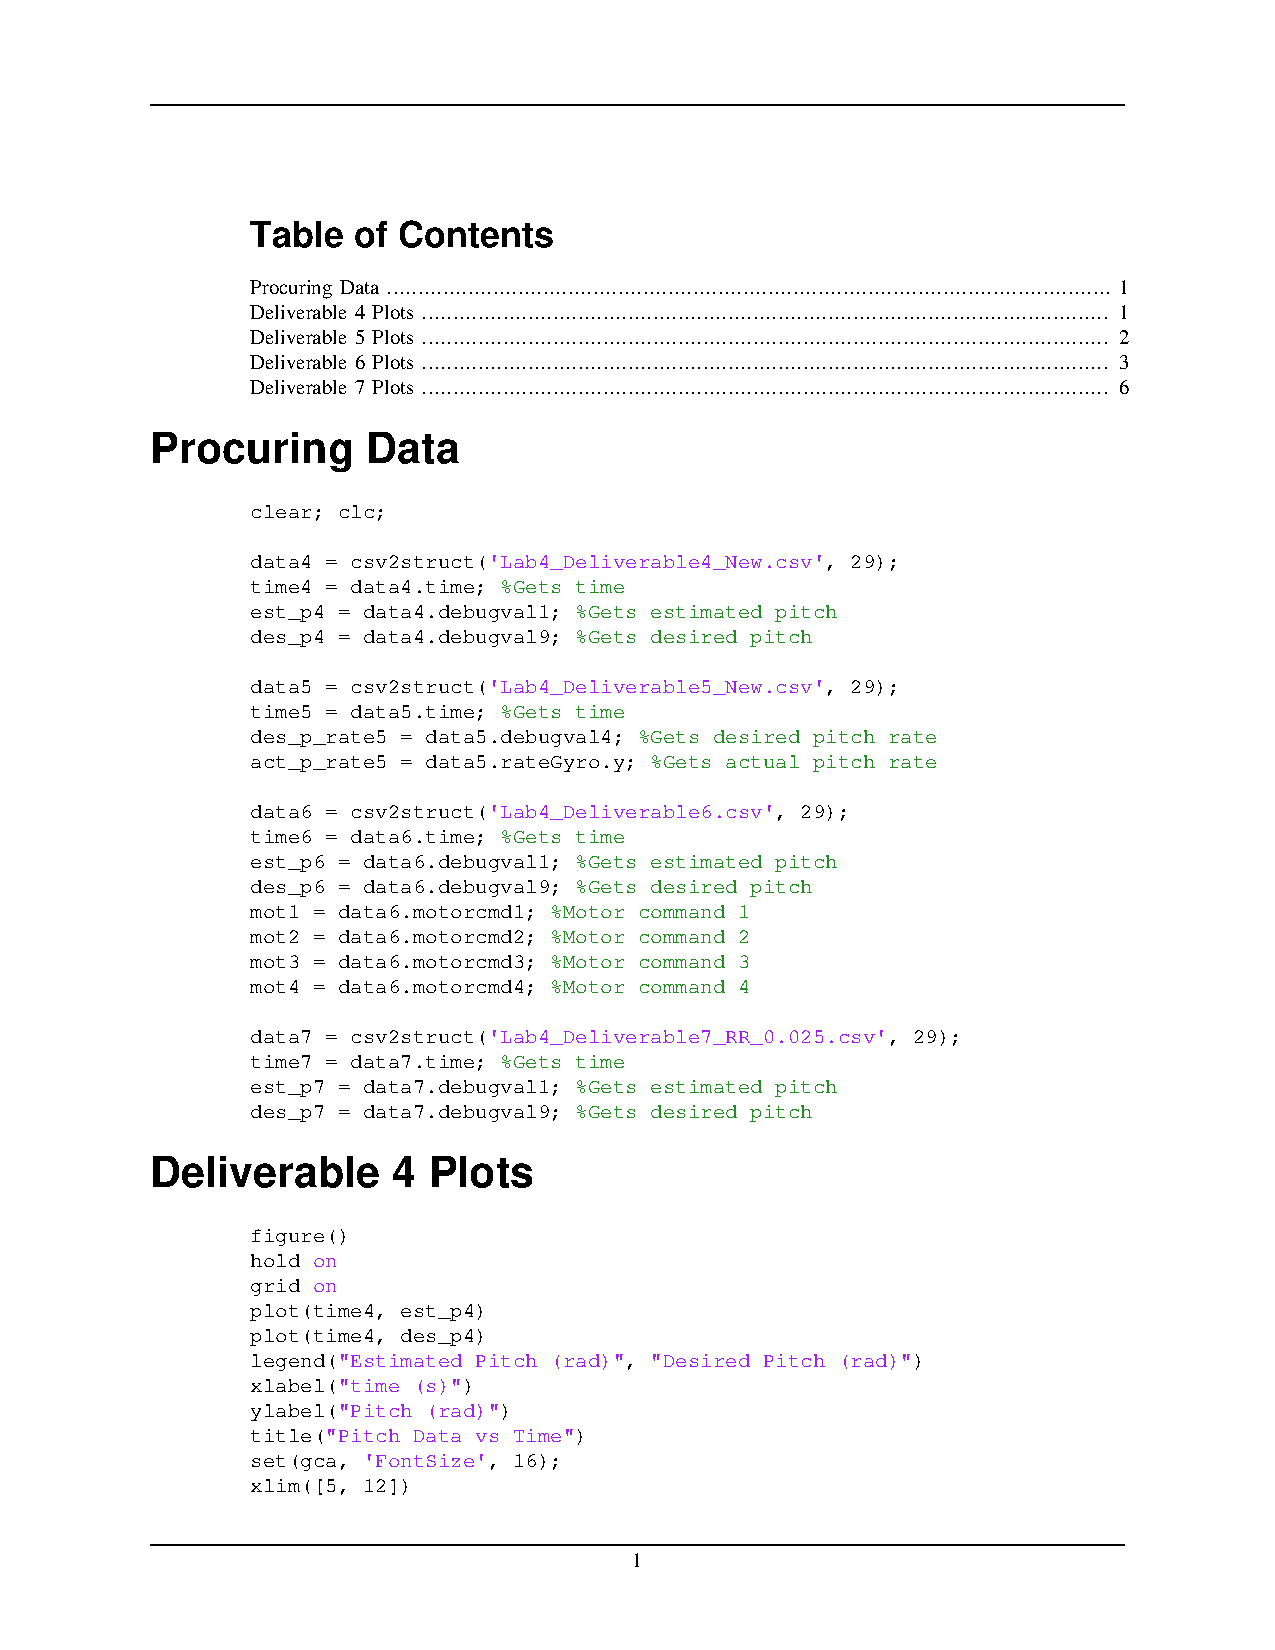
\includepdf[pages=-]{Lab4MatlabCode.pdf} 

\end{document}
